\documentclass{article}

\usepackage{ctex}
\usepackage{graphicx}
\usepackage{float}
\usepackage{amsmath}
\usepackage{amsfonts}
\usepackage{hyperref}

\title{人工智能与游戏第二次作业}
\author{人工智能2101 龚易明}
\date{\today}

\begin{document}

\maketitle

\section{简介}

本次作业先使用Unity设计搭建《逃离丧尸城》游戏,然后在此基础上进一步开发出游戏《明日香的最后一战》。

《逃离丧尸城》游戏和代码已在上次交作业时随邮件附件上交;《明日香的最后一战》文件较大,请从以下链接
下载(这是游戏的发布宣传片,下载链接在评论区):

\href{https://www.bilibili.com/video/BV14T411t7BB}{https://www.bilibili.com/video/BV14T411t7BB}

《明日香的最后一战》代码部分(仅包含个人编写的,不包含更改的资产商店中的代码)在邮件附件中。

以下简要介绍《逃离丧尸城》和《明日香的最后一战》的开发过程,如已经批改过第一次提交的作业(逃离丧尸城),可直接跳到《明日香的最后一战》部分。

\section{逃离丧尸城}

\subsection{游戏设计}

《逃离丧尸城》是一个简单的FPS游戏,游戏中玩家被困在一个港口的高塔上,
整个港口充斥着丧尸。玩家的目标就是从高塔移动到一艘小船处,逃离丧尸城。

\subsection{游戏规则}

游戏中,玩家共有两种武器,一种是突击步枪,一种是半自动步枪。
使用突击步枪击杀一个丧尸需要3枪,使用半自动步枪需要1枪。
玩家子弹有限,而丧尸较多,玩家需要尽可能节约子弹,并避免交火。

玩家不会游泳,如果掉入水中,玩家会直接死亡。
如果玩家从过高的地方跳下,也会摔死。
为增强真实感,游戏还有以下设定:

\begin{enumerate}
    \item 玩家没有血量设定,只要被丧尸碰到就会被感染。
    \item 游戏场景中没有任何弹药补给。
    \item 丧尸移动速度很快(但还是比玩家稍慢)。
    \item 丧尸具有一定智能,看到玩家之前会随机游走,但看到玩家之后就会直接追赶玩家,并且在看不到玩家时会尝试向玩家之前所在的位置移动。
\end{enumerate}

游戏截图如下:

\begin{figure}[H]
    \begin{center}
        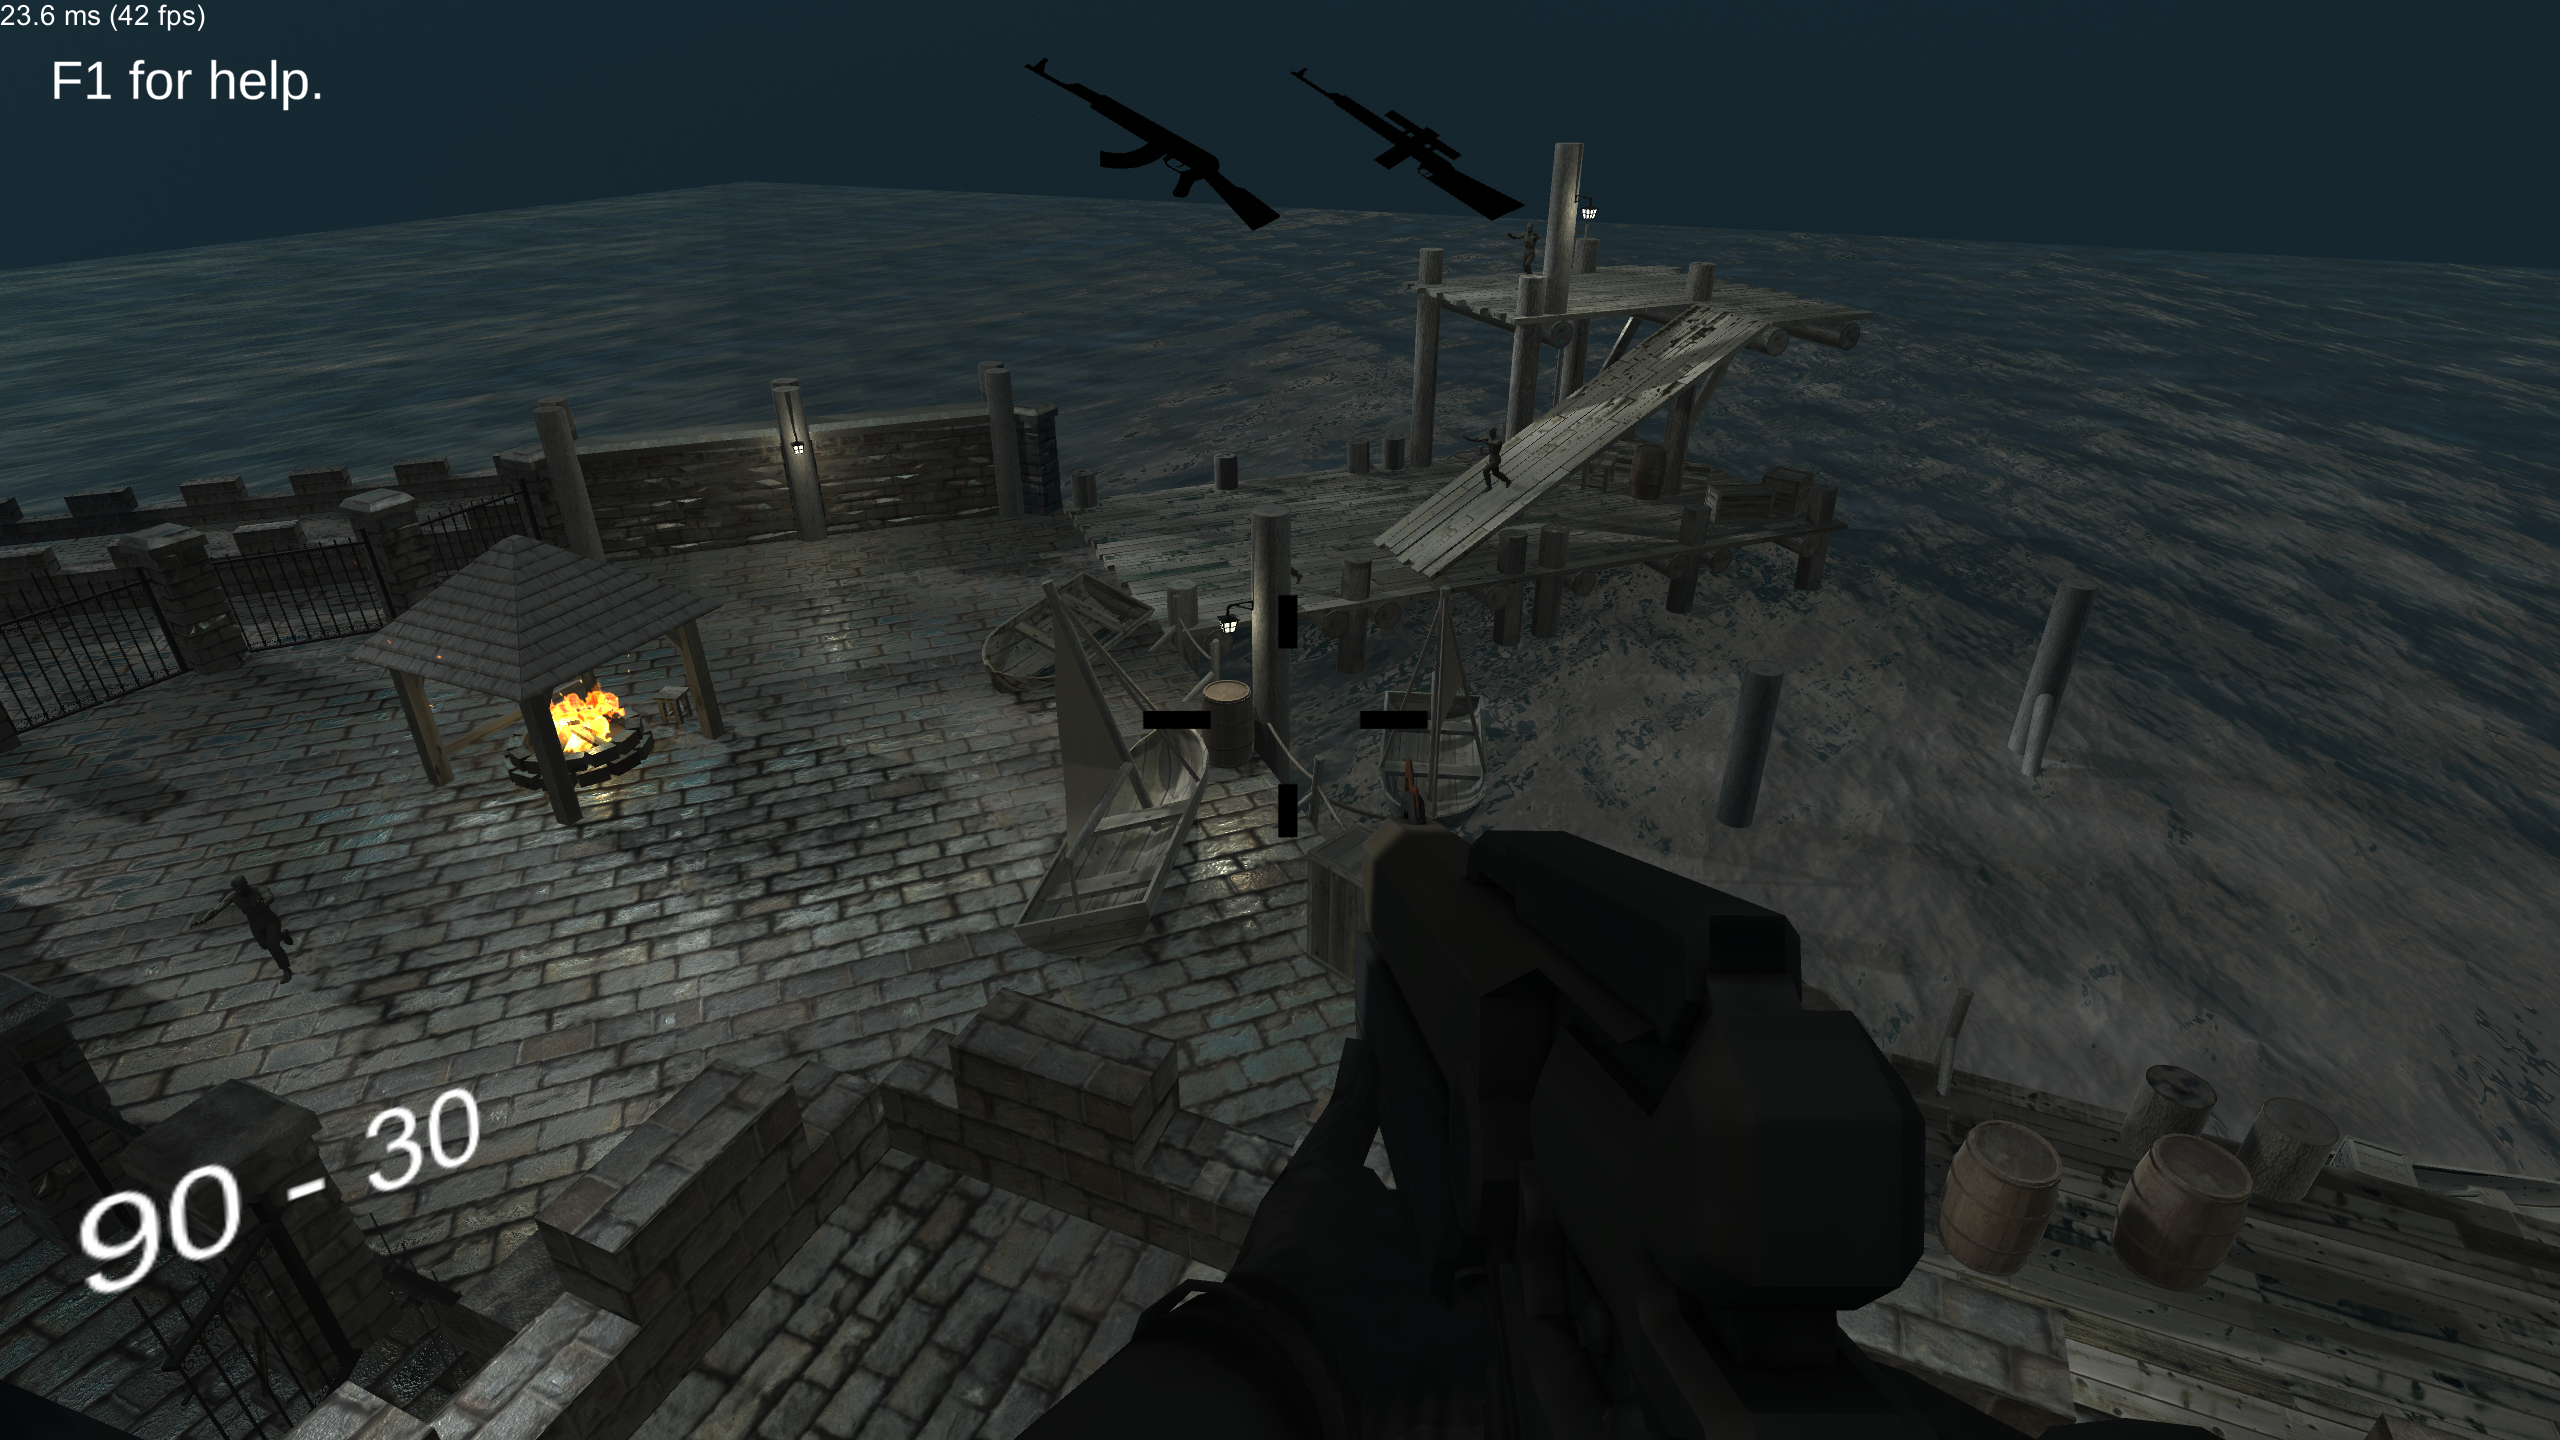
\includegraphics[scale=0.25]{res/screenshot.png}
    \end{center}
\end{figure}

\section{开发过程}

\subsection{免费资产导入}

本次作业使用了Unity Asset Store中的一些免费资源,包括:

\begin{enumerate}
    \item Easy FPS:提供了FPS游戏角色,包括了动画、枪械、手部模型,以及移动、开火和切枪的脚本。
    \item Old Sea Port:提供了丧尸城的场景模型。
    \item Zombie:提供了丧尸的模型和骨骼动画。
    \item TextMesh Pro(Unity自带):提供了向UI添加文字的功能。
\end{enumerate}

\subsection{丧尸行为设计}

这里编写非常简单的丧尸行为脚本。丧尸会尽可能向玩家移动,如果看不到玩家,就会向玩家之前所在的位置移动。

丧尸的寻路(Pathfinding)使用Unity自带的Navmesh系统,这一系统提供了生成从一个点到另一个点的路径的功能。
Unity寻路功能的实现使用了A*算法和避障算法。

游戏中,玩家一直在移动,因此丧尸的移动路径应是一直更新的。由于A*算法的开销较大,
这里为每个丧尸每隔0.5秒计算一次路径。若丧尸能看到玩家,则会记住玩家的位置,向这个位置移动;
若丧尸看不到玩家,则会向玩家之前所在的位置移动。

丧尸移动的脚本为Assets/Scripts/ZombieMoveBehavior.cs。

\subsection{战斗系统}

游戏中,玩家的子弹能对丧尸造成伤害。玩家开枪的脚本由Easy FPS提供,分析其源码后发现玩家每次开枪都会spawn一个bullet对象,
这个对象并不可见,但会检测开枪的方向是否有碰撞体。这里修改了bullet的脚本,增加了判断碰撞体是否为丧尸的功能,
如果为丧尸,就调用丧尸的TakeDamage方法对丧尸造成伤害。

若丧尸血量低于0,就会死亡。丧尸死亡时会通知丧尸的骨骼动画控制器,播放丧尸向后倒地的动画。

与这一功能相关的脚本有Assets/Scripts/Bullet.cs,
Assets/Scripts/TakeDamage Interface.cs,
ZombieTakeDamage.cs。

其中,Assets/Scripts/Bullet.cs为修改后的bullet脚本,其余脚本均为自行编写。

\subsection{玩家死亡逻辑}

游戏中,玩家死亡的可能原因有三种:被丧尸感染而死;掉入水中淹死;从过高的地方跳下摔死。

负责被丧尸感染而死的脚本为Assets/Scripts/PlayerGetInfected.cs。
这一脚本在碰撞检测时检测碰撞到的物体是否为丧尸,如果是丧尸,就激活玩家被感染的UI,
并删除玩家游戏对象。

负责掉入水中淹死的脚本为Assets/Scripts/PlayerDrownBehavior.cs。
这一脚本在碰撞检测时检测碰撞到的物体是否为水,如果是水,就激活玩家淹死的UI,
并删除玩家游戏对象。

负责从过高的地方跳下摔死的脚本为Assets/Scripts/PlayerFallToDeath.cs。
这一脚本在碰撞检测时检测玩家与碰撞体在垂直方向的相对速度,如果相对速度大于一个阈值,
就激活玩家摔死的UI,并删除玩家游戏对象。

\subsection{玩家逃离逻辑}

游戏中,玩家需要从高塔上逃离,逃离的方式是到达一艘小船处。
为判断玩家是否逃离成功,在小船处(小船所在的位置添加了一个粒子系统,产生狼烟的效果,这样玩家就知道小船在哪里了)
设置碰撞体,如果玩家碰到这个碰撞体,就激活玩家逃离成功的UI。
与这一功能相关的脚本为Assets/Scripts/PlayerEscape.cs。
这一脚本在碰撞检测时检测碰撞到的物体是否为小船,如果是小船,就激活玩家逃离成功的UI,
并删除玩家游戏对象。

\subsection{丧尸诞生逻辑}

游戏中设置了5个丧尸点,每个丧尸点每隔5秒会刷出一个丧尸,丧尸点开始刷丧尸的时间为0-5之间的服从均匀分布的一个随机数。
与刷丧尸功能相关的脚本为Assets/Scripts/SpawnZombie.cs。

\subsection{Easy FPS玩家bug修复}

Easy FPS提供的玩家脚本有一个bug,当玩家切换枪械时,枪械的子弹数量会恢复成初始值
(相当于一种作弊器,只要切枪就可以回满子弹)。分析Easy FPS源码后发现,
玩家在切换枪械时会删除当前枪械,并重新生成一把新枪,这就是枪械子弹数复位的原因。
为修复这一bug,更改Easy FPS源码,玩家每次切枪时,若要切换到的枪械没有被生成过,
则生成新枪,但若要切换到的枪械已经被生成过,则直接激活并切换到这把枪。
此外,切枪时不会删除原有枪械,而是将原有枪械设为"disabled"
(Unity中disabled的游戏对象不会被更新,对游戏世界也没有作用)。
这样,枪械就可以保留子弹数目的信息了。

\subsection{UI设计}

这里设计非常简单的UI。游戏的左上角有一个提示信息,提示信息告诉玩家如何显示帮助界面;
玩家按下对应按键时,帮助界面会显示在屏幕上,提示玩家如何操作。
玩家被感染、被淹死、摔死、逃离成功时,会显示相应的UI,告诉玩家游戏结束。
玩家可以重启或退出游戏。

与UI相关的脚本是Assets/Scripts/Manager.cs。

以上自行编写的代码约300行。

\section{明日香的最后一战}

《逃离丧尸城》开发完成并(第一次)提交作业后,
又在此基础上开发出了另一款画质更高、游戏体验更好的游戏:《明日香的最后一战》。

\subsection{游戏设计}

游戏设计的基础是《逃离丧尸城》,但有不少新的功能和设定:

\begin{enumerate}
    \item 玩家的目标变为了消灭所有敌人。
    \item 玩家不会被敌人碰到即判定死亡,而是有血量设定。
    \item 增加了主菜单和暂停菜单。
    \item 增加了近战动作。
    \item 玩家不会摔死。
    \item 玩家的敏捷性大幅提高。
    \item 增加了不同难度设定,从低到高依次为无敌、简单、中等、困难、真实。
    \item 增加了对Linux和macOS的支持。
    \item 使用了HDRP(高质量渲染管线),增加了不同画面质量设定,最高画质支持光线追踪(光线追踪仅支持Windows)。
    \item 增加了一张新地图``学校''。
    \item 敌人模型改为动漫《新世纪福音战士》中的``量产机''。
    \item 玩家模型改为动漫《新世纪福音战士》中的``二号机''。
\end{enumerate}

\subsection{开发流程}

将《逃离丧尸城》升级为《明日香的最后一战》的过程中,做了很多工作,整体开发流程远长于《逃离丧尸城》,
因篇幅原因,这里仅简要介绍各项工作:

\begin{enumerate}
    \item 使用Blender将``量产机''和``二号机''的模型分别骨骼绑定到《逃离丧尸城》中丧尸和玩家模型对应的骨骼上,
    这样就可以直接使用《逃离丧尸城》中丧尸和玩家的动画了。
    \item 修改了玩家的行为脚本,添加了健康值HUD(Health Bar)脚本,记录玩家当前血量,
    玩家被敌人攻击时降低血量。
    \item 修改了丧尸的行为脚本,并添加了控制丧尸骨骼动画的有限状态机,丧尸每隔一段时间可以攻击玩家,
    攻击玩家时停止移动,并播放攻击动画,玩家距离丧尸较远时,每隔一段时间重新计算一次路径,向玩家移动。
    \item 使用了Unity提供的高质量渲染管线(HDRP),并使用了HDRP提供的光线追踪功能。为将游戏升级到HDRP版本,
    将游戏中的所有材质自动升级为了HDRP版本,无法自动升级的手动升级。
    \item 使用Unity资产商店中的``Japanese School''资产,添加了一张新地图``学校''。
    \item 为两张地图分别生成了静态全局光照,并添加了HDRI背景,提高了光照质量。
    \item 使用Unity新版本提供的UI Toolkit(一种类似HTML的UI设计语言),添加了主菜单和暂停菜单。
    可以选择地图、更改游戏难度、画面质量、退出游戏、重新开始游戏等等。
\end{enumerate}

\section{总结}

本次作业使用Unity搭建了一个简单的《逃离丧尸城》游戏平台,并在此基础上开发了游戏《明日香的最后一战》。

\end{document}